\documentclass[12pt]{article}

%% Escrevendo em português:
\usepackage[brazil]{babel}
\usepackage[utf8]{inputenc}
\usepackage[pdftex]{hyperref}
\usepackage{epstopdf}
\usepackage{psfrag}
\usepackage{setspace}
\usepackage{graphicx}
\usepackage{color}
\usepackage{caption}
\usepackage{subcaption}
\usepackage{float}
\usepackage{amsmath}
\usepackage{amsfonts}
\usepackage{amssymb}
%----------------------------


\newtheorem{teorema}{Teorema}%[chapter]
\newtheorem{problema}[teorema]{Problema}
\newtheorem{conj}[teorema]{Conjectura}
\newtheorem{lema}[teorema]{Lema}
\newtheorem{exerc}[teorema]{Exercício}

\definecolor{lightgray}{gray}{0.95}

% Ad hoc macros
\newcommand{\qed}       {\hfill\Box}
\newcommand{\card}[1]   {\left|#1\right|}
\newcommand{\nct}       {\chi_{_T}}
\newcommand{\cnk}[2]    {C_{#1}^{#2}}
\newcommand{\ed}[2]     {#1#2}
\newcommand{\teto}[1]   {\lceil #1 \rceil}
\newcommand{\piso}[1]   {\lfloor #1 \rfloor}
\newcommand{\itab}[1]{\hspace{0em}\rlap{#1}}
\newcommand{\tab}[1]{\hspace{.2\textwidth}\rlap{#1}}

%%%%%%%%%%%%%%%%
\begin{document}
	%%%%%%%%%%%%%%%%
	
\begin{titlepage}
\begin{center}	

\newcommand{\HRule}{\rule{\linewidth}{0.5mm}}
% Upper part of the page. The '~' is needed because \\
% only works if a paragraph has started.

\includegraphics[width=0.15\textwidth]{logoUnicamp}~\\[1cm]

\textsc{\LARGE Universidade Estadual de Campinas}\\[1.5cm]

\textsc{\Large Faculdade de Engenharia Mecânica}\\[0.5cm]

% Title
\HRule \\[0.4cm]
{ \Large \bfseries{ES926 - Automação Industrial\\ \vspace{0.8cm} Projeto Final}\\
\large{Maturação no processo de Fabricação de Cerveja}\\[0.4cm] }

\HRule \\[1.5cm]

% Author and supervisor
\begin{minipage}{0.6\textwidth}
\begin{flushleft} \large
\emph{Nome:}\\
Daniel Dello Russo Oliveira\\ Marcelli Tiemi Kian\\ Vinicius Ragazi David
\end{flushleft}
\end{minipage}
\begin{minipage}{0.2\textwidth}
\begin{flushright} \large
\emph{RA}\\ 101918\\
117892\\ 120258
\end{flushright}
\end{minipage}

\vfill

% Bottom of the page
{\large \today}

\end{center}
\end{titlepage}

	
	\tableofcontents
	%\listoffigures
	%\listoftables
	
	\clearpage
	
	%%%%%%%%%%%%%%%%%%%%%%%%%%%%%%%%%%%%%%%%%%
	\section{Descrição Técnica do Processo}
	
	\begin{par}
		Este relatório consiste na descrição da solução encontrada para o problema da maturação e filtragem da produção de cerveja. O processo começa após a fermentação da cerveja verde que são mandados para os tanques de maturação (válvula VCV e timer1). No tanque a cerveja verde permanece entre 1h e 3h (timer2) com controle constante de sua temperatura, esta necessitando estar em 0ºC, ou no máximo entre -5 e 5ºC. Este controle de temperatura deve ser feito com base no acionamento do fluido refrigerante (VFR) e em um sensor de temperatura (ST).
	\end{par}
	
	\begin{figure}[H]
		\centering
		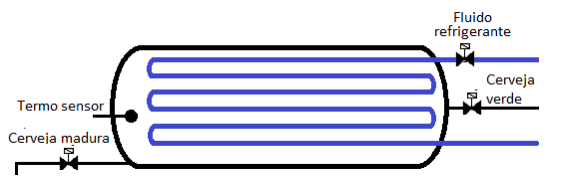
\includegraphics [width=4in]{tanque.png}
		\caption {Tanque de maturação da cerveja verde.}
		\label{fig:corrente}
	\end{figure}
	
	\begin{par}
		Passado este tempo e com sucesso do controle de temperatura a cerveja verde torna-se cerveja madura e é desepeja na próxima etapa (válvula VCM). A etapa consiste em passar por um filtro com terra diatomácea (válvula VTD), que retira partículas desagradáveis à cerveja. 
		
		O resíduo do filtro deve ser descatado após o uso, o seu descarte é feito pela acionamento de uma válvula (VR) que dependerá de um sensor (SBF).
		
		
		Tanto a vávula de despejo da cerveja maturada quanto a da terra diatomácea dependem do sensor de volume do tanque de maturação (SBM).
	\end{par}
	
	\begin{figure}[H]
		\centering
		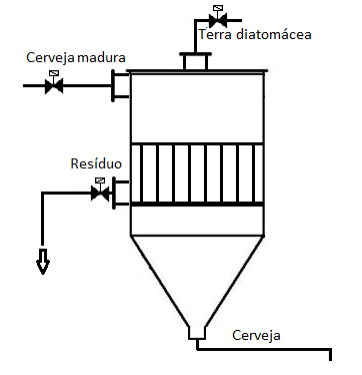
\includegraphics [width=4in]{filtro.png}
		\caption {Filtro da cerveja maturada.}
		\label{fig:corrente}
	\end{figure}
	
	\begin{par}
		Após a filtragem a cerveja é então destinada à próxima etapa da sua fabricação, sendo este não descrito por este trabalho.
	\end{par}
	
	
	\section {Análise do Projeto}
	\begin {itemize}
	\item Modo Automático
	\begin{par}
	
	O modo automático consiste na mudança de estado automática. Quando todas as condições necessárias para a mudança de estado se tornam verdadeiras e o modo automático está ativo a mudança de estado acontecerá, sendo assim, não sendo necessária a atuação humana. Este modo permite um processo mais rápido e mais barato por não necessitar de um funcionário presente para fazer as transições. Contudo poderá haver problemas caso a verificação para as condições estiver com problema, se os sensores, por exemplo, estiverem com problema o processo pode avançar mesmo não sendo o momento apropriado para tal.
	\end{par}
	
	\item Modo Passo a Passo
	
	O modo passo a passo é o oposto do modo automático, sendo assim necessário a atuação humana para a transição de estados. Com todas as condições de transição verdadeiras o processo apenas mudará de estado caso um botão no IHM (interface homem máquina) seja apertado manualmente. Caso ascondições de transição não sejam obdecidas e o operador utilizar o botão do IHM nada acontecerá.
	
	O valor do modo passo a passo é verificado em teste, já que o processo pode ser totaltmente controlado pelo engenheiro de qualidade, testando todas as transições e funcionalidade das entradas (sensores e timers) do sistema.
	
	\item Modo Homming
	
	O modo Homming quando acionado imposibilitará a transição do estado inicial (Home) para o próximo. A transição somente ocorrerá quando o botão "Iniciar" da IHM for apertado. Ele funciona como o modo passo a passo, mas somente para o estado Home, todos os demais funcionam normalmente, estamo no modo passo a passo ou no modo automático.
	
	\item Parada de emergência
	
	
	\item Alarmes e tratamentos de Erros
	
	
	\item IHM
	
	
\end{itemize}

\section {Tabela de designação}
{
\begin {table}
\caption {Tabela de Input.}
\centering
	\begin{tabular}{|  p{2cm} | p{10cm} | p{2cm} | }
\hline
Entrada & Utilidade & Posição\\
\hline
SBM & sensor de volume baixo no tanque de maturação & ??? \\
  ST & sensor de temperatura no tanque de maturação & ??? \\
 SBF & sensor de volume baixo do filtro & ??? \\
\hline
\end{tabular}\\
\end {table}
}


{
\begin {table}
\caption {Tabela de Output.}
\centering
\begin{tabular}{|  p{2cm} | p{10cm} | p{2cm} | }
\hline
Atuador & Utilidade & Posição\\
\hline
  VCV & acionamento da válvula da cerveja verde & ??? \\
  VCM & acionamento da válvula da cerveja maturada & ??? \\
 VFR & acionamento da válvula de fluido refrigerante & ??? \\
VTD & acionamento da válvula de terra diatomácia & ???\\
VR & acionamento da vállvula de discarte & ???\\
 \hline
\end{tabular}\\
\end{table}
}


{
\begin {table}
\caption {Tabela de Temporizadores.}
\centering
\begin{tabular}{|  p{2cm} | p{10cm} | p{2cm} | }
\hline
Nome & Utilidade & Posição\\
\hline
timer1 &  temporizador de entrada da cerveja verde & ??? \\
 timer2 & temporizador da maturação da cerveja verde & ??? \\
 \hline
\end{tabular}
\end{table}
}

\section {Implementação do sistema}


\section {Conclusões}


\begin{thebibliography}{5}
	
	\bibitem{Ogata11} K. Ogata, \emph{Engenharia de Controle Moderno}, 6ª edição, 2011.
	
\end{thebibliography}

\end{document}
